\chapter{Proposta}
A proposta desse trabalho é a elaboração de uma máquina de raciocínio utilizando programação dinâmica e que seja implementada na linguagem Prolog. As entradas da máquina de raciocínio serão: uma localização (X,Y), um tempo restante e uma base de conhecimento que contém as missões ainda não realizadas. A partir dessas entradas, a máquina de raciocínio avaliará quais missões devem ser executadas para que se alcance a quantidade máxima de pontos possível.

A base de conhecimento das missões que ainda não foram realizadas será desenvolvida da seguinte forma: cada fato da base de conhecimento será uma missão, e cada missão terá um tempo de execução e uma pontuação associada. Inicialmente, o tempo para realizar cada missão será fixo, pois o robô sempre partirá da base. A evolução do algoritmo se dará ao adicionar mais variáveis, como por exemplo o tempo de deslocamento do ponto atual, sendo este qualquer ponto no mapa, à outro ponto. Cada evolução será testada com o cenário de uso.

Para determinar o tempo de execução de cada missão, partindo da base, será feito um levantamento dos vídeos da matéria Princípios de Robótica Educacional, onde os alunos realizaram as missões e gravaram em vídeo de forma fiel, sem edição alguma. Serão selecionados apenas os vídeos em que o robô utilizado foi montado de acordo com o indicado pela LEGO. Para cada missão, será feita uma média dos tempos realizados pelos grupos e essa média será assumida como o tempo de execução da missão. No caso de não haver vídeos para alguma missão, a mesma será executada cinco vezes e então será feita a média dos tempos.

O algoritmo terá como saída um roteiro de missões, o qual deverá ser executado pelo robô. O comando para realizar cada missão será enviado via \textit{bluetooth} para o robô, utilizando a ferramenta PLNXT.

\section{Arquitetura do robô}
\apud{vieira2005controle}{rinconframework} define uma arquitetura para robôs móveis baseada em cinco camadas: percepção, decisão, planejamento de caminho, geração de trajetória e sistema de controle. Essa arquitetura pode ser visualizada na Figura \ref{arquiteturaCamadas}.
\clearpage

\FloatBarrier
\begin{figure}[!h]
\centering
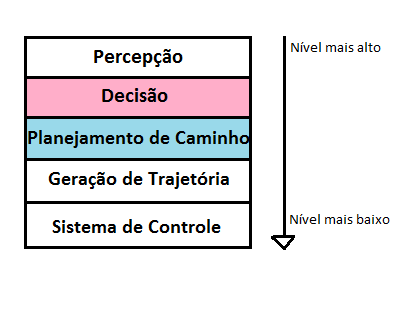
\includegraphics[keepaspectratio=true,scale=0.5]{figuras/arquiteturaCamadas.png}
\caption{Arquitetura em camadas de robôs móveis - \apud{vieira2005controle}{rinconframework}}
\label{arquiteturaCamadas}
\end{figure}

A primeira camada, denominada Camada de Percepção, trata da percepção do robô acerca do mundo ao seu redor, utilizando os sensores que o compõe. Essa camada é responsável, por exemplo, por identificar os obstáculos contidos no tapete.

A segunda camada, denominada Camada de Decisão, é a responsável por decidir as ações que o robô irá executar. Esta camada é o cerébro do robô e será nela que o trabalho proposto irá agir. A máquina de raciocínio que atuará nesta camada terá o cálculo da trajetória, definida na 	quarta camada, através do \textit{framework} Traveller. Conhecendo a trajetória será possível para a maquína de raciocínio calcular o tempo necessário de execução de cada missão e decidir quais missões deverão ser executadas.

A terceira camada define a trajetória que o robô irá executar para chegar à posição desejada, é nessa camada que o \textit{framework} Traveller age. Com o conhecimento do ambiente anteriormente levantado pela Camada de Percepção o Traveller define um percurso por onde o robô deverá seguir e no qual não colidirá com nenhum obstáculo.

A quarta camada recebe o plano da trajetória feito pela camada anterior e define quais ações devem ser feitas sobre o \textit{hardware} para executar o plano. Essa camada tem conhecimento das dimensões e limitações do robô. A última camada atua diretamente no \textit{hardware} para garantir que os atuadores estão recebendo o sinal e agindo conforme planejado.
 
\section{Montagem do robô}
O robô que será utilizado por este trabalho é o Tribot, um tipo de montagem do robô NXT. Nessa montagem, o robô utiliza três motores, um para cada roda e um para a garra que se encontra na parte frontal do robô. O motor da esquerda deve ser ligado na porta C, o da direita na porta B e o da garra na porta A. Essa montagem utiliza também os sensores de toque, de som, de cor e de distância. O tutorial completo, contendo o passo-a-passo para a montagem do robô pode ser encontrado no site da LEGO\footnote{https://education.lego.com/fr-fr/lesi/support/product-support/mindstorms-education-nxt/nxt-base-set-9797/building-instructions}. Na Figura \ref{tribot} é possível visualizar a aparência do robô quando montado. 

\FloatBarrier
\begin{figure}[!h]
\centering
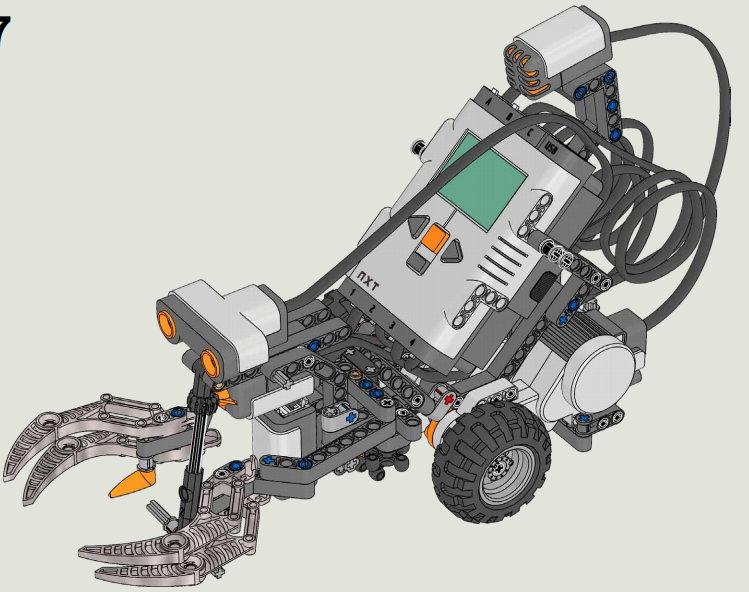
\includegraphics[keepaspectratio=true,scale=0.5]{figuras/tribot.png}
\caption{Montagem do robô Tribot - Lego Mindstorms NXT}
\label{tribot}
\end{figure}


\section{Tapete de missões} \label{tapeteDeMissoes}
O tapete de missões escolhido para ser utilizado por esse trabalho é o \textit{Nature's Fury}, utilizado como desafio do torneio \textit{First Lego League} de 2013, que tem como temática uma tsunami que está devastando as cidades. Nesse tapete, as crianças são ensinadas quanto aos lugares seguros e não seguros para permanecer quando uma tsunami está em atividade. Os lugares seguros durante uma tsunami, demarcados no tapete, são bonificados com uma pontuação extra, caso o robô fique nesse lugar. Já os lugares inseguros também são demarcados no tapete. Porém, esse lugares representam penalidades, com perda de pontuação, caso o robô passe pelos mesmos. Existem missões de salvar os animais de estimação, salvar pessoas, levar água e mantimentos para os lugares seguros.
O tapete \textit{Nature's Fury} foi escolhido para ser objeto de trabalho deste projeto por ser utilizado nas aulas de Princípios de Robótica Educacional, sendo assim, mais acessível do que os outros tapetes. Na Figura \ref{natureFury} é possível visualizar o tapete, bem como os obstáculos que possui. 

\FloatBarrier
\begin{figure}[!h]
\centering
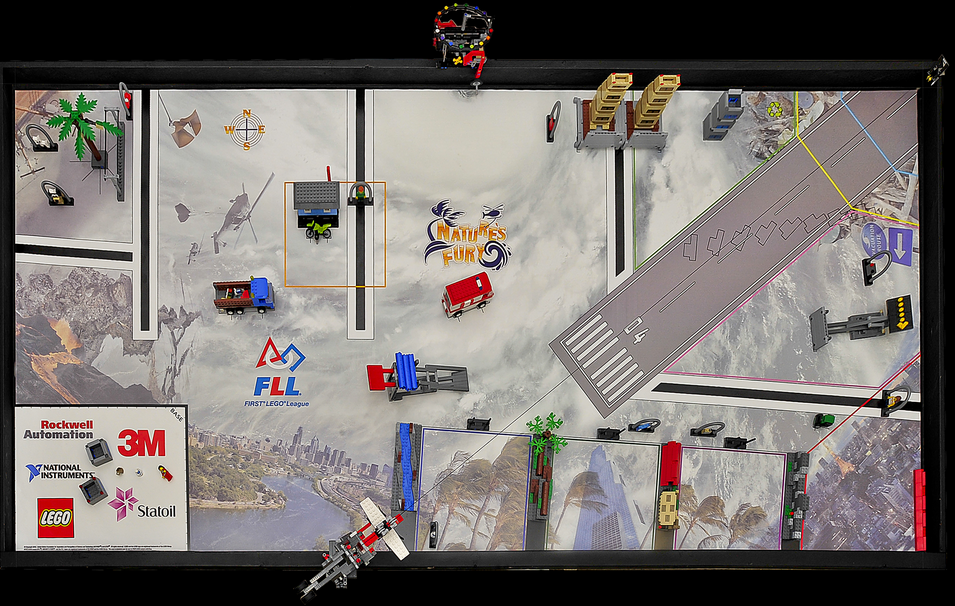
\includegraphics[keepaspectratio=true,scale=0.5]{figuras/natureFury.png}
\caption{Tapete de missões \textit{Nature's Fury} - Lego Mindstorms NXT}
\label{natureFury}
\end{figure}

 
\section{Descrição das missões}
As missões contidas no tapete \textit{Nature's Fury} são descritas a seguir.
\begin{itemize}
\item \textbf{Missão caminhão de fornecimento:} consiste em levar o caminhão até a área amarela do mapa. Pontuação: 20 pontos;
\item \textbf{Missão sinal de evacuação:} consiste em levantar a placa com o sinal de evacuação. Pontuação: 30 pontos;
\item \textbf{Missão avião de carga:} consiste em fazer o avião chegar à área azul ou amarela do tapete. Pontuação: 20 pontos para a área amarela, 30 pontos para a área azul;
\item \textbf{Missão galho da árvore:} consiste em retirar o galho da árvore sem deixá-lo encostar nos fios de alta tensão. Pontuação: 30 pontos;
\item \textbf{Missão tsunami:} consiste em fazer com que as três ondas que estão suspensas toquem o tapete. Pontuação: 20 pontos;
\item \textbf{Missão ambulância:} consiste em levar a ambulância até a área amarela do tapete. Pontuação: 25 pontos;
\item \textbf{Missão pista limpa:} consiste em retirar qualquer objeto da pista de pouso. Pontuação: 30 pontos;
\item \textbf{Missão realocação de construção:} consiste em retirar todas as peças cinzas encontradas na construção da área verde do tapete. Pontuação: 20 pontos;
\item \textbf{Missão teste da base de isolamento:} consiste em encostar na base de isolamento e derrubar apenas um dos prédios. Pontuação: 30 pontos;
\item \textbf{Missão construção:} consiste em empilhar os segmentos na área rosa do tapete. Pontuação: 5 pontos para cada segmento empilhado;
\item \textbf{Missão obstáculo:} consiste no robô passar por cima de obstáculos chegando às áreas coloridas do tapete. Nesse caso, para cada cor do tapete, existe uma pontuação. Pontuação: 10 pontos para a área azul, 16 pontos para a área verde, 23 pontos para a área roxa e 31 pontos para a área vermelha.
\item \textbf{Missão elevar a casa:} consiste no robô abaixar a alavanca que eleva a casa. Pontuação: 25 pontos;
\item \textbf{Missão progresso:} consiste em rodar um círculo de cores. Pontuação: 2 pontos para cada cor que o ponteiro passar.
\item \textbf{Missão família:} consiste em juntar as pessoas que estão no tapete em uma única área colorida. Pontuação: 33 para duas pessoas juntas, ou 66 para 3 pessoas juntas;
\item \textbf{Missão água:} consiste em juntar ao menos uma pessoa com uma garrafa de água na mesma região. Pontuação: 15 pontos para cada pessoa+água;
\item \textbf{Missão segurança:} consiste em levar pelo menos uma pessoa à região vermelha ou amarela do tapete. Pontuação: 12 pontos para cada pessoa na área amarela ou 18 pontos para cada pessoa na área vermelha;
\item \textbf{Missão \textit{pets}:} consiste em juntar ao menos um animal à uma pessoa numa área colorida. Pontuação: 15 pontos para cada pet+pessoa;
\item \textbf{Missão equipamentos e suprimentos:} consiste em levar pelo menos um item, exceto a água, para a região vermelha ou amarela do tapete. Pontuação: 3 pontos para cada item na área amarela ou 4 pontos para cada item na área vermelha;
\item \textbf{Missão lugar seguro:} consiste no robô estar na região vermelha no final do jogo. Pontuação: 25 pontos. 
\end{itemize}

\section{Informações gerais sobre a condução do trabalho}
O desenvolvimento deste trabalho será feito utilizando a metodologia ágil, com \textit{sprints} de em média uma semanas e \textit{releases} a cada duas sprints. No início de cada \textit{sprint}, será feito o planejamento da sprint, definindo as issues que serão realizadas. Cada issue será registrada na ferramenta Waffle, que será integrada ao GitHub.
Para controle de versão do código e da escrita do TCC, foi criada uma organização\footnote{https://github.com/Prolego} no GitHub que contêm dois repositórios: um chamado Prolego\footnote{https://github.com/Prolego/prolego}, para controle de versão do código, e outro chamado Prolego\_doc\footnote{https://github.com/Prolego/prolego\_doc}, para controle de versão da escrita do TCC. Toda a codificação será feita levando em consideração as boas práticas de programação. Na Figura \ref{gitHub} é possível visualizar a organização Prolego criada no GitHub, bem como os repositórios que possui.

\vspace*{1in}

\FloatBarrier
\begin{figure}[!h]
\centering
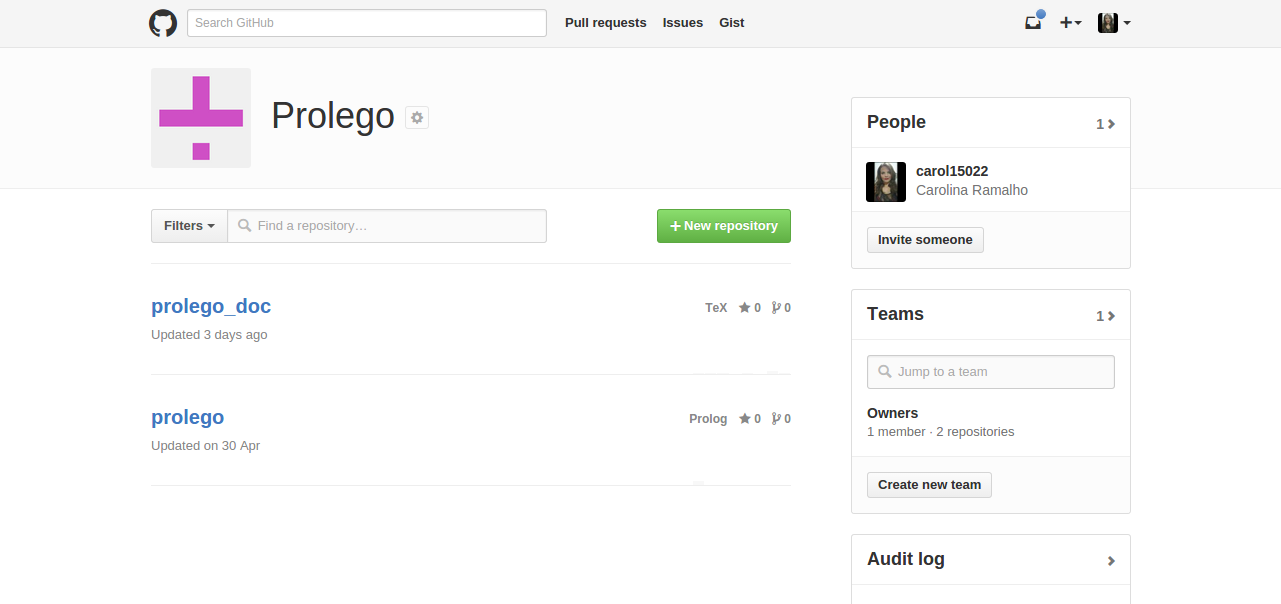
\includegraphics[keepaspectratio=true,scale=0.4]{figuras/gitHub.png}
\caption{Organização Prolego - GitHub}
\label{gitHub}
\end{figure}
\clearpage

\section{Considerações parciais}
A proposta desse trabalho consiste na criação de uma máquina de raciocínio para tomada de decisões estratégicas na robótica educacional, utilizando a linguagem de programação Prolog, a programação dinâmica e o robô Lego Mindstorms NXT. 

Para auxiliar no cálculo do tempo de execução de cada missão, será utilizado o \textit{framework} Traveller, que define a trajetória do robô dado um ponto inicial e um ponto final. A montagem do robô escolhida para ser utilizada por esse trabalho é a Tribot, uma montagem padrão do NXT. O tapete escolhido para ser trabalhado foi o \textit{Nature's Fury}, um dos mais conhecidos e utilizados tapetes da LEGO. 

Para que seja possível a programação do robô na linguagem Prolog, é necessária a utilização da IDE SWI-Prolog. Para a integração do robô com o Prolog, é necessário a instalação da plataforma PLNXT. Ambas as ferramentas são multiplataformas, Linux e Windows, porém nesse trabalho o sistema operacional escolhido foi o Linux.
Todo o trabalho será versionado pelo GitHub e está disponível de forma livre, sendo possível acompanhar todo o desenvolvimento dessa máquina de raciocínio.